\chapter{Beschreibung des Versuchs}

Der Laborversuch besch�ftigt sich mit einer Einf�hrung in die Konfiguration von
Cisco Switches mit dem Cisco \ac{CLI}.

\section{Versuchsaufbau}\label{Aufbau}

% \begin{figure}[ht] 
%   \centering
%      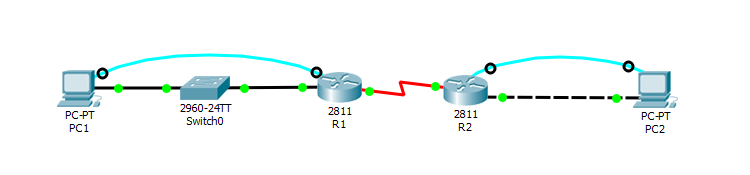
\includegraphics[width=\linewidth]{Graphics/Aufbau.PNG}
%   \caption{Versuchsaufbau}
%   \label{fig:aufbau}
% \end{figure}

\subsection{Komponenten}

% \begin{itemize}
%   \item 2 Computer
%   \begin{itemize}
%     \item HyperTerminal als Emulationsprogramm
%   \end{itemize}
%   \item 2 Cisco 2811 Router
%   \begin{itemize}
%     \item Router 1: 
%     \begin{itemize}
%       \item Verbindung zu PC1 mittels DB-9 zu RJ45 Adapterkabel
%       \item Verbindung zum Switch durch Straight-Through-Kabel
% 	\end{itemize}
% 	\item Router 2:
% 	\begin{itemize}
%     \item Verbindung zu PC2 durch Crossover-Kabel und DB-9 zu RJ45 Adapterkabel
%     \end{itemize}
%     \item Verbindung untereinander durch Serial-Kabel
%   \end{itemize}
%   \item 1 Cisco 2960 Switch
%   	\begin{itemize}
%     	\item Verbindung zu PC1 durch Straight-Through-Kabel
%    	\end{itemize}
% \end{itemize}

\clearpage

\section{Versuchsdurchf�hrung}

\subsection{Teil 1}\label{teil1}

% \begin{table}[!htbp]
% \centering
% \small
% 	\begin{tabularx}{1.05\textwidth}{|X|X|X|X|X|}
% 	\hline
% 	\textbf{Device} & \textbf{Hostname} & \textbf{Interface} & \textbf{IP-Address} &
% 	\textbf{Subnet Mask} \\
% 	\hline
% 	R1 	& R1  & Serial 0/0/0 & 172.17.0.1 & 255.255.0.0 \\
% 	\hline
% 	& & FastEthernet 0/0 & 172.16.0.1 & 255.255.0.0 \\
% 	\hline
% 	R2 & R2 &Serial 0/0/0 & 172.17.0.2 & 255.255.0.0 \\
% 	\hline
% 	 & & FastEthernet 0/0 & 172.18.0.1	& 255.255.0.0 \\
% 	\hline
% 	\end{tabularx}
% \caption{Konfiguration der Router}
% \label{config}
% \end{table}

\underline{Weiteres Vorgehen:}
% \begin{itemize}
%   \item Hostnamen der Router konfigurieren
%   \item Konsole, ``priviledged EXEC mode'' und vty
%   passwords konfigurieren
%   \item Ethernet- und Serial-Schnittstellen konfigurieren
%   \item \ac{MOTD} konfigurieren
%   \item Router so konfigurieren, dass keine Adressaufl�sung f�r Hostnamen
%   durchgef�hrt wird
%   \item Synchrones ``console logging'' konfigurieren
%   \item Verbindung der Hosts und Router �berpr�fen
% \end{itemize}

\subsection{Teil 2}\label{teil2}


\section{Versuchsziel}

